\ifx\enablecjktoken\undefined \scrollmode \expandafter\stop \fi

\RequirePackage{plautopatch}
\documentclass[a5paper,dvipdfmx,14pt]{beamer}
\usepackage{minijs}
\usepackage{newpxtext,newpxmath}
\usepackage{url}
\usepackage{pxjahyper}
\usepackage{hytexconf19} % personal settings

%% customize beamer theme
\makeatletter
%
\usetheme{default}
\setbeamertemplate{section in toc}[sections numbered]
\setbeamertemplate{navigation symbols}{}% removed
\setbeamertemplate{title page}% based on 'default' but slightly modified
{
  \vbox{}
  \vfill\vfill
  \begingroup
    \centering
    \begin{beamercolorbox}[sep=8pt,center]{title}
      \usebeamerfont{title}\inserttitle\par%
      \ifx\insertsubtitle\@empty%
      \else%
        \vskip0.25em%
        {\usebeamerfont{subtitle}\usebeamercolor[fg]{subtitle}\insertsubtitle\par}%
      \fi%
    \end{beamercolorbox}%
    \vskip0.5em\par
    \begin{beamercolorbox}[sep=8pt,center]{author}
      \usebeamerfont{author}\insertauthor
    \end{beamercolorbox}
   \ifx\insertinstitute\@empty\else%
    \begin{beamercolorbox}[sep=8pt,center]{institute}
      \usebeamerfont{institute}\insertinstitute
    \end{beamercolorbox}
   \fi%
    \begin{beamercolorbox}[sep=8pt,center]{date}
      \usebeamerfont{date}\insertdate
    \end{beamercolorbox}\vskip0.5em
    {\usebeamercolor[fg]{titlegraphic}\inserttitlegraphic\par}
  \endgroup
}
%
\usefonttheme{professionalfonts}
\setbeamersize{description width=.8cm}
%
\usecolortheme{default}
\setbeamercolor*{palette primary}{fg=black!80!green,bg=white!90!blue!90!green}
\setbeamercolor*{titlelike}{parent=palette primary}

\renewcommand{\kanjifamilydefault}{\gtdefault}

% misc
\def\cs#1{\texttt{\char92\nobreak#1}}
\def\pTeX{p\kern-.15em\TeX}
\def\upTeX{u\pTeX}
\def\pLaTeX{p\LaTeX}
\def\upLaTeX{u\pLaTeX}

% \scsnowman
\usepackage{scsnowman}
% minimal svgnames from xcolor package
\definecolor{Green}{rgb}{0,0.5,0}
\definecolor{Brown}{rgb}{.648,.165,.165}
\definecolor{SkyBlue}{rgb}{.53,.808,.92}
\definecolor{DarkGoldenrod}{rgb}{.72,.525,.044}
\def\SCSNOWMAN{\scsnowman[scale=2,adjustbaseline,
  muffler=red,hat=Green,arms=Brown,snow=SkyBlue,buttons=DarkGoldenrod]}

\usepackage{tcolorbox}

\begin{document}

%% 1
\title{\pTeX のペナルティ}
\author{山下 弘展}
\date{2019年10月12日\\\TeX Conf 2019}
\begin{frame}
  \maketitle
\end{frame}

%% 2
\begin{frame}{はじめに:ペナルティとは}
\begin{tcolorbox}[colframe=black!70!green,colback=white!90!blue!90!green,
  coltitle=white,fonttitle=\bfseries,
  title=\TeX におけるペナルティ(penalty)]
  行分割時やページ分割時に
  「その箇所がブレークポイントとしてどの程度適切であるか」
  を示す評価値.
\end{tcolorbox}
\leavevmode\null\par
\pTeX では,和文組版に必須の禁則処理を実現するために拡張されている.\par\bigskip
{\footnotesize
 ※ \pTeX にはもう一つ,パラグラフの最終行が和文文字一字で孤立するのを防ぐ
 \cs{jcharwidowpenalty}というペナルティもあるが,本講演では時間の都合上取り扱わない.}
\end{frame}

%% 3 (verbatim -> fragile)
\begin{frame}[fragile]{前提}
\begin{itemize}
\item \pTeX~p3.8.2 (\TeX\ Live 2019)ベース
\item 特に断らない限り,初期設定を仮定
{\small
\begin{verbatim}
  % 禁則ペナルティ
  \prebreakpenalty`.=10000
  \prebreakpenalty`。=10000
  \postbreakpenalty`(=10000
  \postbreakpenalty`(=10000
  % 一文字だけの行を抑制
  \jcharwidowpenalty=500
\end{verbatim}
}
\end{itemize}
\end{frame}

%% 4
\begin{frame}{禁則処理とペナルティ}
\begin{tcolorbox}[colframe=black!70!green,colback=white!90!blue!90!green,
  coltitle=white,fonttitle=\bfseries,
  title=組版規則]
\begin{itemize}\leftskip-15pt
\item 欧文:連続する文字列=単語の途中では行分割が起こらない\null\footnotemark
\item 和文:ほとんどの文字間が分割可能.
  この例外が\COLOREMPH{禁則}(行頭/行末禁則).
\end{itemize}
\end{tcolorbox}
\footnotetext{ハイフネーション処理等の特別な場合を除く.}
\pause
\pTeX の実装では…
\begin{itemize}
\item 各文字間を分割可能に=\underline{グルー}の自動挿入\\
      \phantom{各文字間を分割可能に}{\footnotesize \cs{kanjiskip}, \cs{xkanjiskip}}
\item 禁則処理=\underline{\COLOREMPH{ペナルティ}}の自動挿入\\
      \phantom{禁則処理}{\footnotesize 禁則テーブルに基づく}
\end{itemize}
\end{frame}

%% 5
\begin{frame}[fragile]{参考:NTT \JTeX との比較}
\pTeX の実装では…
\begin{itemize}
\item 各文字間を分割可能に=\underline{グルー}の自動挿入\\
      \phantom{各文字間を分割可能に}{\footnotesize \cs{kanjiskip}, \cs{xkanjiskip}}
\item 禁則処理=\underline{\COLOREMPH{ペナルティ}}の自動挿入\\
      \phantom{禁則処理}{\footnotesize 禁則テーブルに基づく}
\end{itemize}
\leavevmode\null\par
\JTeX の実装では…
\begin{itemize}
\item 各文字間を分割可能に=\underline{グルー}の自動挿入\\
      \phantom{各文字間を分割}{\footnotesize \cs{jintercharskip}, \cs{jasciikanjiskip}}
\item 禁則処理=\COLOREMPH{グルーの自動挿入を抑制}\null
      \footnote{記号類とひらがな,カタカナについてのみ指定可.}
\end{itemize}
\end{frame}

%% 6
\begin{frame}{\pTeX の禁則処理の基礎}
\pTeX は\COLOREMPH{禁則テーブル}に従い,
\COLOREMPH{ペナルティ}を文字の前後適切な位置に自動挿入する.
\begin{tcolorbox}[colframe=black!70!green,colback=white!90!blue!90!green,
  coltitle=white,fonttitle=\small\bfseries,
  title=禁則テーブル(KINSOKU table)]\small
\begin{itemize}\small\leftskip-5pt\baselineskip0pt
  \item 禁則対象とする文字のコード
  \item その文字に対するペナルティ値
  \item ペナルティの挿入位置(行頭禁則ならその文字の前に挿入,行末禁則なら後)
\end{itemize}
を登録できる(最大256文字まで).
\end{tcolorbox}
\pause
テーブルへの登録・削除用プリミティブ:
\begin{center}
  \cs{prebreak{\color{red}penalty}}, \cs{postbreak{\color{red}penalty}}
\end{center}
\end{frame}

%% 7
\begin{frame}[fragile]{\pTeX の禁則処理の基礎}
\pTeX の標準設定では
\begin{itemize}\small
\item 約物(句読点やカッコ類)
\item 小書き仮名
\end{itemize}
等が禁則テーブルに登録されている.
{\footnotesize
\begin{verbatim}
  例:
  \prebreakpenalty`。=10000    %  "。" の前に10000
  \postbreakpenalty`(=10000   %  "(" の後に10000
  \prebreakpenalty`ゃ=150      %  "ゃ" の前に150
\end{verbatim}
}
しかし,ユーザが自由に登録・削除・値を変更することもできるようになっている\null
\footnote{実際に削除できるようになったのは,コミュニティ版p3.8.1以降.}.
\end{frame}

%% 8
\begin{frame}[fragile]{\pTeX の禁則処理の制約事項}
\begin{enumerate}\setcounter{enumi}{0}
\item \underline{禁則の指定は文字コードに依る}\\[1ex]
  {\small
    禁則テーブルには和文文字と欧文文字の区別なく登録できるが,
    登録されるのは「文字」そのものではなく「\COLOREMPH{文字コード}」である.\\
    $\rightarrow$
    \pTeX では和文文字の内部コードは2バイト,
    欧文文字は1バイトであるから衝突しない.\\
    \upTeX では和文文字(CJK)の内部コードが
    欧文文字(8-bit Latin)に被ることがある:
  \begin{itemize}% newpx defaults to T1
    \item \texttt{0xA1}:\quad \kchar"A1 (CJK) vs. \char"A1\ (8-bit Latin)
    \item \texttt{0xAB}:\quad \kchar"AB (CJK) vs. \char"AB\ (8-bit Latin)
    \item \texttt{0xB7}:\quad \kchar"B7 (CJK) vs. \char"B7\ (8-bit Latin)
  \end{itemize}
  “一方を立てれば一方が立たず”\\
   \hskip2zw=前者を禁則扱いすれば,後者も禁則扱いに}
\end{enumerate}
\end{frame}

%% 9
\begin{frame}[fragile]{\pTeX の禁則処理の制約事項}
\begin{enumerate}\setcounter{enumi}{1}
\item \underline{行頭禁則と行末禁則は同時指定不可}\\[1ex]
  {\small
    同一の文字コードに対して,
    \cs{prebreakpenalty}と\cs{postbreakpenalty}の両方を
    \COLOREMPH{同時に与えるような指定はできない}.
    もし両方指定された場合,\COLOREMPH{後から指定されたもの}に置き換えられる.
{\footnotesize
\begin{verbatim}
  例:
  \prebreakpenalty`〜=10000
  \showthe\prebreakpenalty`〜  % => 10000
  \showthe\postbreakpenalty`〜 % => 0
  \postbreakpenalty`〜=10000
  \showthe\prebreakpenalty`〜  % => 0
  \showthe\postbreakpenalty`〜 % => 10000
\end{verbatim}
}}
\end{enumerate}
\end{frame}

%% 10
\begin{frame}{本題}
\begin{center}
ここまでがアスキーによる「仕様」.\par\bigskip
しかし,いくつか注意したい点がある.
\end{center}
\end{frame}

\section{欧文文字に対する禁則処理の課題}

%% 11
\begin{frame}[fragile]{\insertsectionnumber. \insertsection}
禁則テーブルには和文文字と欧文文字の区別なく登録できるが,
実際には細かい注意が必要.\medskip

\dbendrule\bigskip
\pause
\pTeX がボックスを構築する様子を明らかにするため,
\cs{showlists}や\cs{showbox}といったプリミティブを活用.\medskip

{\small
ボックスの中身を完全に表示するためのおまじない:
\begin{verbatim}
    \tracingonline  = 1
    \showboxdepth   = 10000
    \showboxbreadth = 10000
\end{verbatim}
}
\end{frame}

\subsection{禁則ペナルティの挿入タイミング}\label{penaget}

\def\ruleKINSOKUjp{%
\begin{tcolorbox}[colframe=black!70!green,colback=white!90!blue!90!green,
  coltitle=white,fonttitle=\small\bfseries,
  title=和文文字の場合]\small
禁則ペナルティは,\COLOREMPH{その文字ノードをリストに追加する際}に一緒に挿入される.
\end{tcolorbox}}

%% 12-1
\begin{frame}[t,fragile]{\insertsectionnumber.\insertsubsectionnumber. \insertsubsection}
\ruleKINSOKUjp
{\footnotesize
例:\upTeX で和文フォント\code{upjisr-h}を選択した状況
\begin{itemize}
  \item \verb+\font\x=upjisr-h \x+\\
        \verb+\setbox0=\vbox{です。\showlists}+
\begin{verbnote}
\begin{verbatim}
 \x で
 \x す
 \penalty 10000(for kinsoku)
 \x 。
 \glue(refer from jfm) 5.0
\end{verbatim}
\end{verbnote}
\end{itemize}\vskip-25pt
→ \codechar{。}の前に\cs{prebreakpenalty}由来のペナルティ10000が入った
}
\end{frame}

%% 12-2
\begin{frame}[t,fragile]{\insertsectionnumber.\insertsubsectionnumber. \insertsubsection}
\ruleKINSOKUjp
{\footnotesize
例:\upTeX で和文フォント\code{upjisr-h}を選択した状況
\begin{itemize}
  \item \verb+\font\x=upjisr-h \x+\\
        \verb+\setbox0=\vbox{まず(\showlists}+
\begin{verbnote}
\begin{verbatim}
 \x ま
 \x ず
 \glue(refer from jfm) 5.0 minus 5.0
 \x (
 \penalty 10000(for kinsoku)
\end{verbatim}
\end{verbnote}
\end{itemize}\vskip-25pt
→ \codechar{(}の後に\cs{postbreakpenalty}由来のペナルティ10000が入った
}
\end{frame}

%% 13
\begin{frame}[t,fragile]{\insertsectionnumber.\insertsubsectionnumber. \insertsubsection}
\ruleKINSOKUjp
{\small → この仕様から導かれる挙動(定理):}\smallskip
\begin{tcolorbox}[colframe=black!70!blue,colback=white!90!blue]\small
\begin{itemize}\small\leftskip-18pt\baselineskip0pt
  \item 和文文字の\cs{postbreakpenalty}は
    \COLOREMPH{「現在のリストの最後」になりうる}ため,
    \cs{lastpenalty}で値を取得できるし,\cs{unpenalty}で取り除くこともできる.
  \item 和文文字の\cs{prebreakpenalty}は
    原理的に\COLOREMPH{必ず後ろに文字ノードを伴う}ため,
    挿入後にその値を取得したり取り除いたりすることは\COLOREMPH{できない}.
\end{itemize}
\end{tcolorbox}
\end{frame}

%% 14
\begin{frame}[fragile]{\insertsectionnumber.\insertsubsectionnumber. \insertsubsection}{}
{\footnotesize
例:和文文字の\cs{postbreakpenalty}の取得
\begin{itemize}
  \item \verb+\font\x=upjisr-h \x+\\
        \verb+\setbox0=\vbox{まず(\showthe\lastpenalty}+
\begin{verbnote}
\begin{verbatim}
 > 10000.
\end{verbatim}
\end{verbnote}
\end{itemize}\vskip-20pt
例:和文文字の\cs{postbreakpenalty}の削除
\begin{itemize}
  \item \verb+\font\x=upjisr-h \x+\\
        \verb+\setbox0=\vbox{まず(\unpenalty\showlists}+
\begin{verbnote}
\begin{verbatim}
 \x ま
 \x ず
 \glue(refer from jfm) 5.0 minus 5.0
 \x (
\end{verbatim}
\end{verbnote}
\end{itemize}\vskip-25pt
}
\end{frame}

\def\ruleKINSOKUal{%
\begin{tcolorbox}[colframe=black!70!green,colback=white!90!blue!90!green,
  coltitle=white,fonttitle=\small\bfseries,
  title=欧文文字の場合]\small
禁則ペナルティは,\COLOREMPH{禁則対象の欧文文字が和文文字と
隣り合う場合にのみ}挿入される.\ruleKINSOKUalsub
\end{tcolorbox}}
\def\ruleKINSOKUalsub{つまり,欧文のみの組版では挿入されない(Knuthの\TeX と互換).}

%% 15-1
\begin{frame}[t,fragile]{\insertsectionnumber.\insertsubsectionnumber. \insertsubsection}
\ruleKINSOKUal
{\footnotesize\def\verbnotesize{\scriptsize}
例:\upTeX でさらに欧文フォント\code{cmr10}を選択した状況
\begin{itemize}
  \item \verb+\font\x=upjisr-h \x  \font\A=cmr10 \A+\\
        \verb+\setbox0=\vbox{だるま.\showlists}+
\begin{verbnote}
\begin{verbatim}
 \x だ
 \x る
 \x ま
 \penalty 10000(for kinsoku)
 \A .
\end{verbatim}
\end{verbnote}
\end{itemize}\vskip-25pt
→ 和文\codechar{ま}-欧文\codechar{.}間に,
  \codechar{.}由来の\cs{prebreakpenalty}が入った
}
\end{frame}

%% 15-2
\begin{frame}[t,fragile]{\insertsectionnumber.\insertsubsectionnumber. \insertsubsection}
\ruleKINSOKUal
{\footnotesize\def\verbnotesize{\scriptsize}
例:\upTeX でさらに欧文フォント\code{cmr10}を選択した状況
\begin{itemize}
  \item \verb+\font\x=upjisr-h \x  \font\A=cmr10 \A+\\
        \verb+\setbox0=\vbox{A dog.\showlists}+
\begin{verbnote}
\begin{verbatim}
 \A A
 \glue 3.33333 plus 1.66498 minus 1.11221
 \A d
 \A o
 \A g
 \A .
\end{verbatim}
\end{verbnote}
\end{itemize}\vskip-25pt
→ 欧文\codechar{g}-欧文\codechar{.}間には\cs{prebreakpenalty}が入らない
}
\end{frame}

%% 15-3
\begin{frame}[t,fragile]{\insertsectionnumber.\insertsubsectionnumber. \insertsubsection}
\ruleKINSOKUal
{\footnotesize\def\verbnotesize{\scriptsize}
例:\upTeX でさらに欧文フォント\code{cmr10}を選択した状況
\begin{itemize}
  \item \verb+\font\x=upjisr-h \x  \font\A=cmr10 \A+\\
        \verb+\setbox0=\vbox{A dog.}\showbox0+
\begin{verbnote}
\begin{verbatim}
 ..\A A
 ..\glue 3.33333 plus 1.66498 minus 1.11221
 ..\A d
 ..\A o
 ..\A g
 ..\A .
\end{verbatim}
\end{verbnote}
\end{itemize}\vskip-25pt
→ ボックスを組み終わっても\cs{prebreakpenalty}は入らない
}
\end{frame}

%% 15-4
\begin{frame}[t,fragile]{\insertsectionnumber.\insertsubsectionnumber. \insertsubsection}
\ruleKINSOKUal
{\footnotesize\def\verbnotesize{\scriptsize}
例:\upTeX でさらに欧文フォント\code{cmr10}を選択した状況
\begin{itemize}
  \item \verb+\font\x=upjisr-h \x  \font\A=cmr10 \A+\\
        \verb+\setbox0=\vbox{(だるま\showlists}+
\begin{verbnote}
\begin{verbatim}
 \A (
 \penalty 10000(for kinsoku)
 \x だ
 \x る
 \x ま
\end{verbatim}
\end{verbnote}
\end{itemize}\vskip-25pt
→ 欧文\codechar{(}-和文\codechar{だ}間に,
  \codechar{(}由来の\cs{postbreakpenalty}が入った
}
\end{frame}

%% 15-5
\begin{frame}[t,fragile]{\insertsectionnumber.\insertsubsectionnumber. \insertsubsection}
\ruleKINSOKUal
{\footnotesize\def\verbnotesize{\scriptsize}
例:\upTeX でさらに欧文フォント\code{cmr10}を選択した状況
\begin{itemize}
  \item \verb+\font\x=upjisr-h \x  \font\A=cmr10 \A+\\
        \verb+\setbox0=\vbox{(dog\showlists}+
\begin{verbnote}
\begin{verbatim}
 \A (
 \A d
 \A o
 \A g
\end{verbatim}
\end{verbnote}
\end{itemize}\vskip-25pt
→ 欧文\codechar{(}-欧文\codechar{d}間には\cs{postbreakpenalty}が入らない
}
\end{frame}

%% 16
\begin{frame}[fragile]{\insertsectionnumber.\insertsubsectionnumber. \insertsubsection}
\ruleKINSOKUal
%\begin{itemize}
%  \item 欧文文字直後が和文文字の場合に限り,
%    その欧文文字に対する\cs{postbreakpenalty}を挿入する.
%  \item 欧文文字直前が和文文字の場合に限り,
%    その欧文文字に対する\cs{prebreakpenalty}を挿入する.
%\end{itemize}
{\small → 隣接する文字が重要なので…}\smallskip
\begin{tcolorbox}[colframe=black!70!blue,colback=white!90!blue]\small
\begin{itemize}\small\leftskip-18pt
  \item 欧文文字の\cs{postbreakpenalty}は
    \COLOREMPH{後続の和文文字ノード追加時}に挿入される
    (欧文文字自身と同時ではない).\\
    → \COLOREMPH{「リストの最後」になりえず},
    \cs{lastpenalty}で取得できないし,\cs{unpenalty}でも消せない.
  \item 欧文文字の\cs{prebreakpenalty}は和文と同様.
\end{itemize}
\end{tcolorbox}
\end{frame}

%% 17
\begin{frame}[fragile]{\insertsectionnumber.\insertsubsectionnumber. \insertsubsection}{}
{\footnotesize\def\verbnotesize{\scriptsize}
例:欧文文字の\cs{postbreakpenalty}の削除(失敗)
\begin{itemize}
  \item \verb+\font\x=upjisr-h \x  \font\A=cmr10 \A+\\
        \verb+\setbox0=\vbox{(だるま\showlists}+
\begin{verbnote}
\begin{verbatim}
 \A (
 \penalty 10000(for kinsoku)
 \x だ
 \x る
 \x ま
\end{verbatim}
\end{verbnote}
\end{itemize}\vskip-25pt
\begin{itemize}
  \item \verb+\font\x=upjisr-h \x  \font\A=cmr10 \A+\\
        \verb+\setbox0=\vbox{(\unpenalty だるま\showlists}+
\begin{verbnote}
\begin{verbatim}
 \A (
 \penalty 10000(for kinsoku)
 \x だ
 \x る
 \x ま
\end{verbatim}
\end{verbnote}
\end{itemize}\vskip-25pt
\pause
→ 問題とまではいえないが,使うときは注意が必要.
}
\end{frame}

\subsection{グループ境界での禁則ペナルティ}\label{penagroup}
\def\ruleKINSOKUalsub{}

%% 18
\begin{frame}[t,fragile]{\insertsectionnumber.\insertsubsectionnumber. \insertsubsection}
\ruleKINSOKUal
…はずだが,現在の\pTeX では
\COLOREMPH{グループ境界 \code{\{} や \code{\}} で隔てられた場合}に
欧文文字の禁則ペナルティが{\SUSHI}\underline{入ったり入らなかったり}{\SUSHI}する.
\pause
\begin{itemize}\small
  \item ベースライン補正が0のとき:
    \begin{itemize}\leftskip-10pt
      \item \cs{postbreakpenalty}は大丈夫らしい
      \item \cs{prebreakpenalty}はグループ境界で失敗{\SUSHI}
    \end{itemize}
  \item ベースライン補正が0でないとき:
    \begin{itemize}\leftskip-10pt
      \item \cs{postbreakpenalty}も\cs{prebreakpenalty}も,グループ境界で失敗{\SUSHI}
    \end{itemize}
\end{itemize}
\end{frame}

% \cs{displace}は和欧文のベースライン補正を実現するノード.
% \cs{displace 3.0}は垂直下に3.0\,ptだけシフトし,
% \cs{displace 0.0}で元の位置に戻している.

%% 19-1
\begin{frame}[t,fragile]{\insertsectionnumber.\insertsubsectionnumber. \insertsubsection}{}
{\small
\verb+\ybaselineshift=0pt+の場合:
\begin{itemize}
  % \font\x=upjisr-h \x
  \item \verb+\setbox0=\vbox{(漢({漢}{(}漢\showlists}+
\begin{verbnote}
\begin{verbatim}
 \displace 0.0
 \A (
 \penalty 10000(for kinsoku)
 \x 漢
 \A (
 \penalty 10000(for kinsoku)
 \x 漢
 \A (
 \penalty 10000(for kinsoku)
 \x 漢
\end{verbatim}
\end{verbnote}
\end{itemize}\vskip-25pt
欧文文字の\cs{postbreakpenalty}は問題なさそう
}
\end{frame}

%% 19-2
\begin{frame}[t,fragile]{\insertsectionnumber.\insertsubsectionnumber. \insertsubsection}{}
{\small
\verb+\ybaselineshift=0pt+の場合:
\begin{itemize}
  % \font\x=upjisr-h \x
  \item \verb+\setbox0=\vbox{漢.{漢}.漢{.}\showlists}+
\begin{verbnote}
\begin{verbatim}
 \displace 0.0
 \x 漢
 \penalty 10000(for kinsoku)
 \A .
 \x 漢
 \A .
 \x 漢
 \A .
\end{verbatim}
\end{verbnote}
\end{itemize}\vskip-25pt
欧文文字の\cs{prebreakpenalty}は\COLOREMPH{グループ境界が挟まると挿入されない}?
}
\end{frame}

%% 19-3
\begin{frame}[t,fragile]{\insertsectionnumber.\insertsubsectionnumber. \insertsubsection}{}
{\small\def\verbnotesize{\scriptsize}
\verb+\ybaselineshift=3pt+の場合:
\begin{itemize}
  % \font\x=upjisr-h \x
  \item \verb+\setbox0=\vbox{(漢({漢}{(}漢\showlists}+
\begin{verbnote}
\begin{verbatim}
 \displace 3.0
 \A (
 \penalty 10000(for kinsoku)
 \displace 0.0
 \x 漢
 \displace 3.0
 \A (
 \displace 0.0
 \x 漢
 \displace 3.0
 \A (
 \displace 0.0
 \x 漢
\end{verbatim}
\end{verbnote}
\end{itemize}\vskip-25pt
今度は\cs{postbreakpenalty}も\COLOREMPH{グループ境界でNG}?
}
\end{frame}

%% 19-4
\begin{frame}[t,fragile]{\insertsectionnumber.\insertsubsectionnumber. \insertsubsection}{}
{\small\def\verbnotesize{\scriptsize}
\verb+\ybaselineshift=3pt+の場合:
\begin{itemize}
  % \font\x=upjisr-h \x
  \item \verb+\setbox0=\vbox{漢.{漢}.漢{.}\showlists}+
\begin{verbnote}
\begin{verbatim}
 \displace 0.0
 \x 漢
 \penalty 10000(for kinsoku)
 \displace 3.0
 \A .
 \displace 0.0
 \x 漢
 \displace 3.0
 \A .
 \displace 0.0
 \x 漢
 \displace 3.0
 \A .
 \displace 0.0
\end{verbatim}
\end{verbnote}
\end{itemize}\vskip-25pt
やはり\cs{prebreakpenalty}は\COLOREMPH{グループ境界でNG}?
}
\end{frame}

\subsection{リガチャに対する禁則ペナルティ}\label{penalig}
\font\Q=cmr10 at 12pt

%% 20
\begin{frame}[t,fragile]{\insertsectionnumber.\insertsubsectionnumber. \insertsubsection}
リガチャ(合字)といえば:
\begin{itemize}\small
  \item $\codechar{f}+\codechar{i}$\hspace{37pt}で\hspace{5pt}
    \codechar{\Q f{}i} ではなく \codechar{\Q fi}
  \item $\codechar{f}+\codechar{f}+\codechar{i}$\hspace{7pt}で\hspace{4pt}
    \codechar{\Q f{}f{}i} ではなく \codechar{\Q ffi}
\end{itemize}
など,\COLOREMPH{ある並びの2文字以上が合体して1文字に}
{\footnotesize\def\verbnotesize{\scriptsize}
\begin{itemize}
  \item \verb+\font\x=upjisr-h \x  \font\A=cmr10 \A+\\
        \verb+\setbox0=\vbox{f i fi ffi\showlists}+
\begin{verbnote}
\begin{verbatim}
 \A f
 \glue 3.33333 plus 1.66666 minus 1.11111
 \A i
 \glue 3.33333 plus 1.66666 minus 1.11111
 \A ^^L (ligature fi)
 \glue 3.33333 plus 1.66666 minus 1.11111
 \A ^^N (ligature ffi)
\end{verbatim}
\end{verbnote}
\end{itemize}\vskip-20pt
}
→ 元とは違う\COLOREMPH{単一の文字コード}に置き換わる
\end{frame}

%% 21
\begin{frame}[t,fragile]{\insertsectionnumber.\insertsubsectionnumber. \insertsubsection}
禁則ペナルティを設定したくなるリガチャ:
\begin{itemize}\small
  \item $\codechar{'}+\codechar{'}$\hspace{7pt}で\hspace{4pt}
    \codechar{\Q '{}'} ではなく \codechar{\Q ''}
  \item $\codechar{`}+\codechar{`}$\hspace{7pt}で\hspace{4pt}
    \codechar{\Q `{}`} ではなく \codechar{\Q ``}
\end{itemize}
\medskip
→ さて,禁則ペナルティはどう設定すればよい?\par\medskip
\pause
現在の\pTeX では…
\begin{tcolorbox}[colframe=black!70!blue,colback=white!90!blue]\small
\begin{itemize}\small\leftskip-18pt
  \item \cs{postbreakpenalty}は
    \COLOREMPH{リガチャ自体の文字コード}から決まる.
  \item \cs{prebreakpenalty}はリガチャ自体ではなく,
    \COLOREMPH{それを構成する最初の要素文字コード}から決まる.
\end{itemize}
\end{tcolorbox}
\pause
\leavevmode\hbox to\textwidth{\hfill {\SUSHI}ややこしい{\SUSHI}\hfill}
\end{frame}

%% 22-1
\begin{frame}[t,fragile]{\insertsectionnumber.\insertsubsectionnumber. \insertsubsection}{}
{\small\def\verbnotesize{\scriptsize}
例:\upLaTeX でT1エンコーディングを仮定
\begin{itemize}
  \item $\codechar{>}+\codechar{>}$は合字\codechar{»}を作る.
    \begin{itemize}
      \item 合字の文字コードは \verb|^^T| の位置.
      \item Unicodeでは \verb|U+00BB| にあたる.
    \end{itemize}
\end{itemize}
}
{\small ここで次の入力を考えると…}
{\footnotesize
\begin{verbatim}
    \documentclass{article}
    \usepackage[utf8]{inputenc} % LaTeX 既定
    \usepackage[T1]{fontenc}
    \prebreakpenalty`\^^T=2560
    \prebreakpenalty`\>=128
    \begin{document}
    \setbox0=\hbox{あ>> い\char`\^^T う»}\showbox0
\end{verbatim}
}
{\small → 3回\codechar{»}が出力されるが,ペナルティ値は不統一\SUSHI}
\end{frame}

%% 22-2
\begin{frame}[fragile]{\insertsectionnumber.\insertsubsectionnumber. \insertsubsection}{}
{\footnotesize\def\verbnotesize{\scriptsize}
\begin{itemize}
  \item \verb+\setbox0=\hbox{あ>> い\char`\^^T う»}\showbox0+
\begin{verbnote}
\begin{verbatim}
 .\displace 0.0
 .\x あ
 .\penalty 128(for kinsoku)
 .\glue(\xkanjiskip) 2.5 plus 2.5 minus 1.25
 .\A ^^T (ligature >>)
 .\glue 2.5 plus 1.99997 minus 1.00006
 .\x い
 .\penalty 2560(for kinsoku)
 .\A ^^T
 .\x う
 .\penalty 2560(for kinsoku)
 .\A ^^T
\end{verbatim}
\end{verbnote}
\end{itemize}\vskip-20pt
\begin{itemize}\leftskip20pt
  \item $\codechar{>}+\codechar{>}$の合字(\code{あ}の後):
    \COLOREMPH{要素} \codechar{>} に由来する128
  \item 文字コード直接指定(\code{い}の後):
    {\color{blue}合字} \codechar{>>} に由来する2560
  \item UTF-8入力(\code{う}の後):
    {\color{blue}合字} \codechar{>>} に由来する2560
\end{itemize}
→ 現れるすべての\codechar{»}を行頭禁則にするには,
{\catcode`\^=12 \codechar{>}と\codechar{^^T}}の両方に
\cs{prebreakpenalty}を設定しないといけない\SUSHI
}
\end{frame}

%% 23
\begin{frame}[fragile]{もっとややこしい話}
欧文文字と和文文字の連続箇所は処理が複雑.
\begin{itemize}\small
  \item 禁則ペナルティ
    \begin{itemize}\footnotesize\leftskip-10pt
      \item 挿入される値は「\cs{post...}は\COLOREMPH{リガチャ自体},
        \cs{pre...}は最初の\COLOREMPH{構成要素}」で決まる{\SUSHI}
    \end{itemize}
  \item 和文文字のJFM由来グルー・カーン
  \item 欧文文字のTFM由来カーン
  \item ベースライン補正用ノード
  \item 和欧文間の四分アキ (\cs{xkanjiskip})
    \begin{itemize}\footnotesize\leftskip-10pt
      \item 挿入可否は
        「和文文字に隣接する\COLOREMPH{構成要素}の\cs{xspcode}」で決定{\SUSHI}
    \end{itemize}
\end{itemize}
{\small → しかも,\COLOREMPH{どの順番で挿入するか}も割と問題.}\par\medskip
{\footnotesize
グループ境界(1.\ref{penagroup})とリガチャ(1.\ref{penalig})の挙動については,
\href{https://github.com/texjporg/tex-jp-build/issues/85}{GitHub}にて
\verb+kinsoku_around_word+ブランチまたは
\verb+kinsoku_ligature+ブランチで検討中だが,未完成
}
\end{frame}

\section{和文文字に対する禁則処理}

%% 24
\begin{frame}{\insertsectionnumber. \insertsection}
\pTeX の和欧文混植は難しい{\SUSHI}\par\bigskip
しかし,和文文字の禁則処理についてもいくつかの課題が残っている.
\end{frame}

\subsection{和文文字の禁則ペナルティ取得}

%% 25
\begin{frame}[t]{\insertsectionnumber.\insertsubsectionnumber. \insertsubsection}{}
{\small
1.\ref{penaget}で述べた
\begin{tcolorbox}[colframe=black!70!blue,colback=white!90!blue]\small
\begin{itemize}\small\leftskip-18pt\baselineskip0pt
  \item 和文文字の\cs{postbreakpenalty}は「現在のリストの最後」になりうるため,
    \COLOREMPH{\cs{lastpenalty}で値を取得できるし,\cs{unpenalty}で取り除くこともできる}.
\end{itemize}
\end{tcolorbox}
の「少々デリケートな挙動」の話.
}
\end{frame}

%% 26-1
\begin{frame}[t,fragile]{\insertsectionnumber.\insertsubsectionnumber. \insertsubsection}{}
{\footnotesize
\code{min10}系(\pTeX),\code{jis}系(\file{jsclasses}),\code{upjis}系(\upTeX)のJFMの場合
\begin{itemize}
  \item \verb+\font\x=upjisr-h \x+\\
        \verb+\setbox0=\vbox{あ(\showthe\lastpenalty}+
\begin{verbnote}
\begin{verbatim}
 > 10000.
\end{verbatim}
\end{verbnote}
\end{itemize}\vskip-20pt
\begin{itemize}
  \item \verb+\font\x=upjisr-h \x+\\
        \verb+\setbox0=\vbox{あ(\unpenalty\showthe\lastpenalty}+
\begin{verbnote}
\begin{verbatim}
 > 0.   % 元々 10000 あったものが消えた
\end{verbatim}
\end{verbnote}
\end{itemize}\vskip-20pt
\begin{itemize}
  \item \verb+\font\x=upjisr-h \x+\\
        \verb+\setbox0=\vbox{あ(\ifnum\lastpenalty=10000 \T \fi}+
\begin{verbnote}
\begin{verbatim}
 ! Undefined control sequence. \T
\end{verbatim}
\end{verbnote}
\end{itemize}\vskip-20pt
}
\end{frame}

%% 26-2
\begin{frame}[t,fragile]{\insertsectionnumber.\insertsubsectionnumber. \insertsubsection}{}
{\footnotesize
\file{jlreq}クラスのJFMの場合
\begin{itemize}
  \item \verb+\font\X=ujlreq \X+\\
        \verb+\setbox0=\vbox{あ(\showthe\lastpenalty}+
\begin{verbnote}
\begin{verbatim}
 > 0.   % あれっ?
\end{verbatim}
\end{verbnote}
\end{itemize}\vskip-20pt
\begin{itemize}
  \item \verb+\font\X=ujlreq \X+\\
        \verb+\setbox0=\vbox{あ(\unpenalty\showthe\lastpenalty}+
\begin{verbnote}
\begin{verbatim}
 > 0.   % 元々0だったので \unpenalty とは関係ない
\end{verbatim}
\end{verbnote}
\end{itemize}\vskip-20pt
\begin{itemize}
  \item \verb+\font\X=ujlreq \X+\\
        \verb+\setbox0=\vbox{あ(\ifnum\lastpenalty=10000 \T \fi}+
\begin{verbnote}
\begin{verbatim}
 ! Undefined control sequence. \T  % 0なら出ないはず
\end{verbatim}
\end{verbnote}
\end{itemize}\vskip-20pt
}
\end{frame}

%% 27-1
\begin{frame}[t,fragile]{\insertsectionnumber.\insertsubsectionnumber. \insertsubsection}{}
{\footnotesize\def\verbnotesize{\scriptsize}
\code{min10}系(\pTeX),\code{jis}系(\file{jsclasses}),\code{upjis}系(\upTeX)のJFMの場合
\begin{itemize}
  \item \verb+\font\x=upjisr-h \x+\\
        \verb+\setbox0=\vbox{あ(\showlists}+
\begin{verbnote}
\begin{verbatim}
 \x あ
 \glue(refer from jfm) 5.0 minus 5.0
 \x (
 \penalty 10000(for kinsoku)
\end{verbatim}
\end{verbnote}
\end{itemize}\vskip-20pt
\begin{itemize}
  \item \verb+\font\x=upjisr-h \x+\\
        \verb+\setbox0=\vbox{あ(\unpenalty\showlists}+
\begin{verbnote}
\begin{verbatim}
 \x あ
 \glue(refer from jfm) 5.0 minus 5.0
 \x (
\end{verbatim}
\end{verbnote}
\end{itemize}\vskip-20pt
→ リストの最後が\cs{penalty}ノードなので取得・削除可
}
\end{frame}

%% 27-2
\begin{frame}[t,fragile]{\insertsectionnumber.\insertsubsectionnumber. \insertsubsection}{}
{\footnotesize\def\verbnotesize{\scriptsize}
\file{jlreq}クラスのJFMの場合:\COLOREMPH{\codechar{(}の後にJFMグルーを設定}
\begin{itemize}
  \item \verb+\font\X=ujlreq \X+\\
        \verb+\setbox0=\vbox{あ(\showlists}+
\begin{verbnote}
\begin{verbatim}
 \X あ
 \glue(refer from jfm) 5.0 minus 5.0
 \X (
 \penalty 10000(for kinsoku)
 \glue(refer from jfm) 0.0
\end{verbatim}
\end{verbnote}
\end{itemize}\vskip-20pt
\begin{itemize}
  \item \verb+\font\X=ujlreq \X+\\
        \verb+\setbox0=\vbox{あ(\unpenalty\showlists}+
\begin{verbnote}
\begin{verbatim}
 \X あ
 \glue(refer from jfm) 5.0 minus 5.0
 \X (
 \penalty 10000(for kinsoku)
 \glue(refer from jfm) 0.0
\end{verbatim}
\end{verbnote}
\end{itemize}\vskip-20pt
→ \cs{penalty}ノードより後にJFMグルーがあるので取得・削除に失敗
}
\end{frame}

%% 27-3
\begin{frame}[t,fragile]{\insertsectionnumber.\insertsubsectionnumber. \insertsubsection}{}
\begin{tcolorbox}[colframe=black!70!green,colback=white!90!blue!90!green,
  coltitle=white,fonttitle=\small\bfseries,
  title=\pTeX のJFMグルー挿入規則]
\begin{itemize}\footnotesize\leftskip-18pt
  \item 同じ箇所では「禁則ペナルティ → \underline{JFMグルー}」の順に挿入\\
    \phantom{同じ箇所では「禁則ペナルティ}{\scriptsize JFMグルーのほうが後}
  \item \underline{展開不能トークン}が来たら,文字タイプ0とみなしてJFMグルー挿入
    \hspace{15pt}{\scriptsize \cs{relax},\cs{showthe},\cs{unpenalty},代入も該当}
\end{itemize}
\end{tcolorbox}
\pause
{\footnotesize\def\verbnotesize{\scriptsize}
\file{jlreq}クラスのJFMの場合:\COLOREMPH{\codechar{(}の後にJFMグルーを設定}
\begin{itemize}\leftskip-10pt
  \item \verb+\setbox0=\vbox{あ(\ifnum\lastpenalty>0 \T \fi}+
\begin{verbnote}
\begin{verbatim}
 ! Undefined control sequence. \T
\end{verbatim}
\end{verbnote}
\end{itemize}\vskip-20pt
\qquad → \cs{ifnum}の展開(=判定)時点でグルー挿入はまだ!
\begin{itemize}\leftskip-10pt
  \item \verb+\setbox0=\vbox{あ(\relax\ifnum\lastpenalty>0 \T \fi}+
\begin{verbnote}
\begin{verbatim}
 % エラーなし
\end{verbatim}
\end{verbnote}
\end{itemize}\vskip-20pt
\qquad → 展開不能トークン\cs{relax}の時点でグルーが挿入された\par
}
\end{frame}

%% 28
\begin{frame}[t,fragile]{\insertsectionnumber.\insertsubsectionnumber. \insertsubsection}{}
{\small {\SUSHI} \pLaTeX カーネル(\file{plcore.ltx})より {\SUSHI}}
{\scriptsize
\begin{verbatim}
\def\footnotetext{%
  \ifhmode\pltx@foot@penalty\lastpenalty\unpenalty\fi  % ここで取得→削除
  \@ifnextchar [\@xfootnotenext
    {\protected@xdef\@thefnmark{\thempfn}%
     \@footnotetext}}
\long\def\@footnotetext#1{%
  \ifydir\def\@tempa{\yoko}\else\def\@tempa{\tate}\fi
  \insert\footins{\@tempa%
    ... 中略 ...
    \color@begingroup
      \@makefntext{%
        \rule\z@\footnotesep\ignorespaces#1\@finalstrut\strutbox}%
    \color@endgroup}\ifhmode\null\fi
    \ifnum\pltx@foot@penalty=\z@\else
      \penalty\pltx@foot@penalty                       % ここで復帰
      \pltx@foot@penalty\z@
    \fi}
\end{verbatim}
}
{\small
→ \file{jlreq}クラスでは思うように動いていない\SUSHI\par
\COLOREMPH{取得・削除という操作自身が展開不能なため}\par
}
\end{frame}

\subsection{禁則ペナルティの合算}

\def\ruleKINSOKUadd{%
\begin{tcolorbox}[colframe=black!70!blue,colback=white!90!blue,
  coltitle=white,fonttitle=\small\bfseries,
  title=\pTeX の禁則ペナルティ挿入]
\begin{itemize}\footnotesize\leftskip-18pt
  \item \cs{prebreakpenalty}は,既にその位置にペナルティがあれば
    それに\COLOREMPH{合算}する形で発行される(別には発行されない).
  \item \cs{postbreakpenalty}は,直後に(\cs{prebreakpenalty}以外の)
    ペナルティが来ても合算されず,常に\COLOREMPH{別々}に発行される.
\end{itemize}
\end{tcolorbox}}

%% 29-1
\begin{frame}[t,fragile]{\insertsectionnumber.\insertsubsectionnumber. \insertsubsection}{}
\ruleKINSOKUadd
\pause
{\footnotesize\def\verbnotesize{\scriptsize}
\begin{itemize}
  \item \verb+\setbox0=\vbox{あ)\showlists}+
\begin{verbnote}
\begin{verbatim}
 \x あ
 \penalty 10000(for kinsoku)    % => 10000
 \x )
\end{verbatim}
\end{verbnote}
\end{itemize}\vskip-20pt
\begin{itemize}
  \item \verb+\setbox0=\vbox{()\showlists}+
\begin{verbnote}
\begin{verbatim}
 \x (
 \penalty 20000(for kinsoku)    % => 10000 + 10000 = 20000
 \x )
\end{verbatim}
\end{verbnote}
\end{itemize}\vskip-20pt
}
\end{frame}

%% 29-2
\begin{frame}[t,fragile]{\insertsectionnumber.\insertsubsectionnumber. \insertsubsection}{}
{\footnotesize\def\verbnotesize{\scriptsize}
例:\cs{prebreakpenalty}の前に明示的な\cs{penalty}を入れてみる
\begin{itemize}
  \item \verb+\setbox0=\vbox{あ\penalty5000 )\showlists}+
\begin{verbnote}
\begin{verbatim}
 \x あ
 \penalty 15000               % => 5000 + 10000 = 15000
 \x )
\end{verbatim}
\end{verbnote}
\end{itemize}\vskip-20pt
\pause
\begin{itemize}
  \item \verb+\setbox0=\vbox{あ\break )\showlists}+
\begin{verbnote}
\begin{verbatim}
 \x あ
 \penalty 0                   % => -10000 + 10000 = 0
 \x )
\end{verbatim}
\end{verbnote}
\end{itemize}\vskip-15pt
→ \cs{break}すなわち\cs{penalty -10000}を入れても強制改行できない{\SUSHI}\par\medskip
→ 合算されるのを見越して\cs{penalty -20000}を入れのも面倒{\SUSHI}…\par
}
\end{frame}

%% 30
\begin{frame}[t]{今日のトピックまとめ}{}
  \leavevmode\hbox to\textwidth{\hfill
    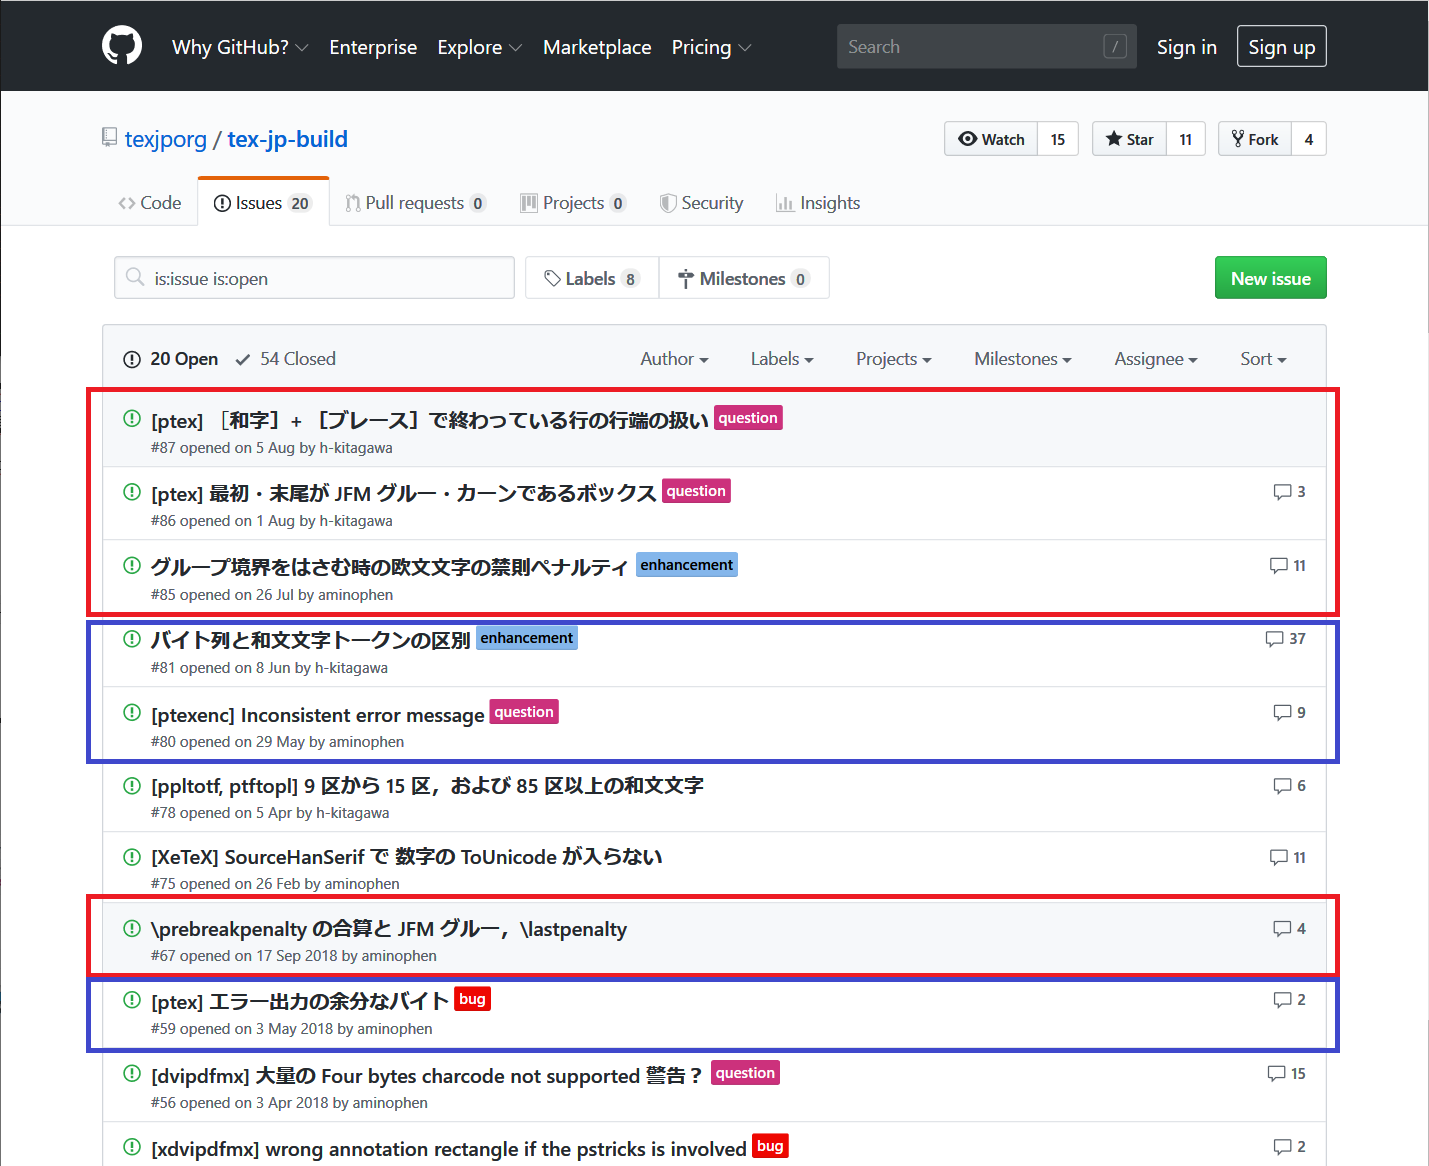
\includegraphics[width=.9\textwidth]{img/20191008_texjpbuild_issues.png}\hfill}
  \par\vskip-105pt
  \pause
\begin{tcolorbox}[colframe=red,colback=white!90!red]\small
  GitHubでいろいろ議論中.ご意見あれば\par
    \url{https://github.com/texjporg/tex-jp-build}\par
  のIssuesまで.
\end{tcolorbox}
\end{frame}

\end{document}
